\documentclass{article}
\usepackage{graphicx}
\usepackage{float}
\usepackage[margin=.75in]{geometry}

\begin{document}

\section{4.2.a+b}

The following set of plots correspond to emulation of system E,ES,S,P as specified in 4.1. Code can be found at github.com/cfmcginn/SystBio/HW1. C++ and ROOT needed to run. A directory containing the set of pdfs used in this document is available at the git repository, along with the .tex used to create this, if wanted individually. Time steps of simulation are .0001, sampling done such that 1000 bins appear on the plot. Simulations show little deviation with variation of time steps up and down an order of magnitude.

\begin{figure}[H]
    \centering
    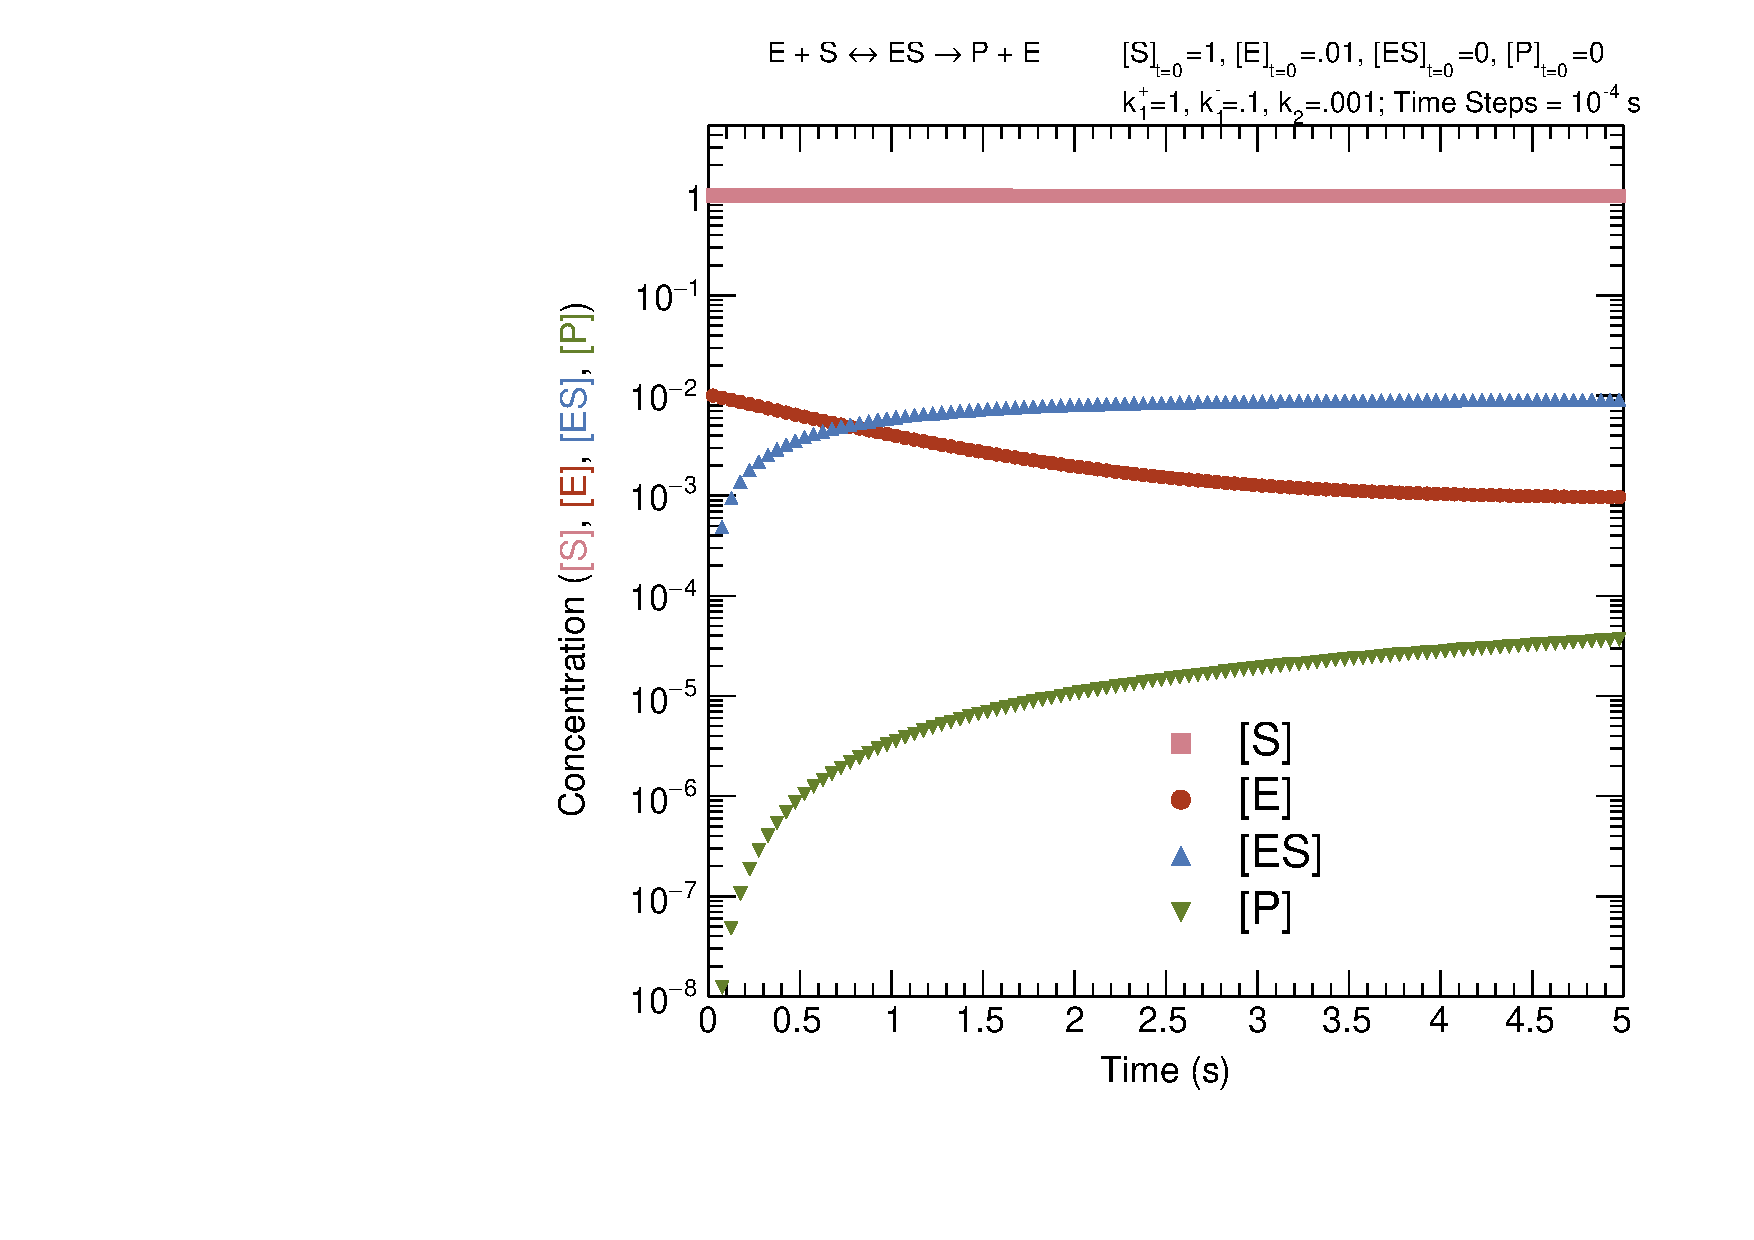
\includegraphics[width=.49\textwidth]{canv5_c.pdf} 
    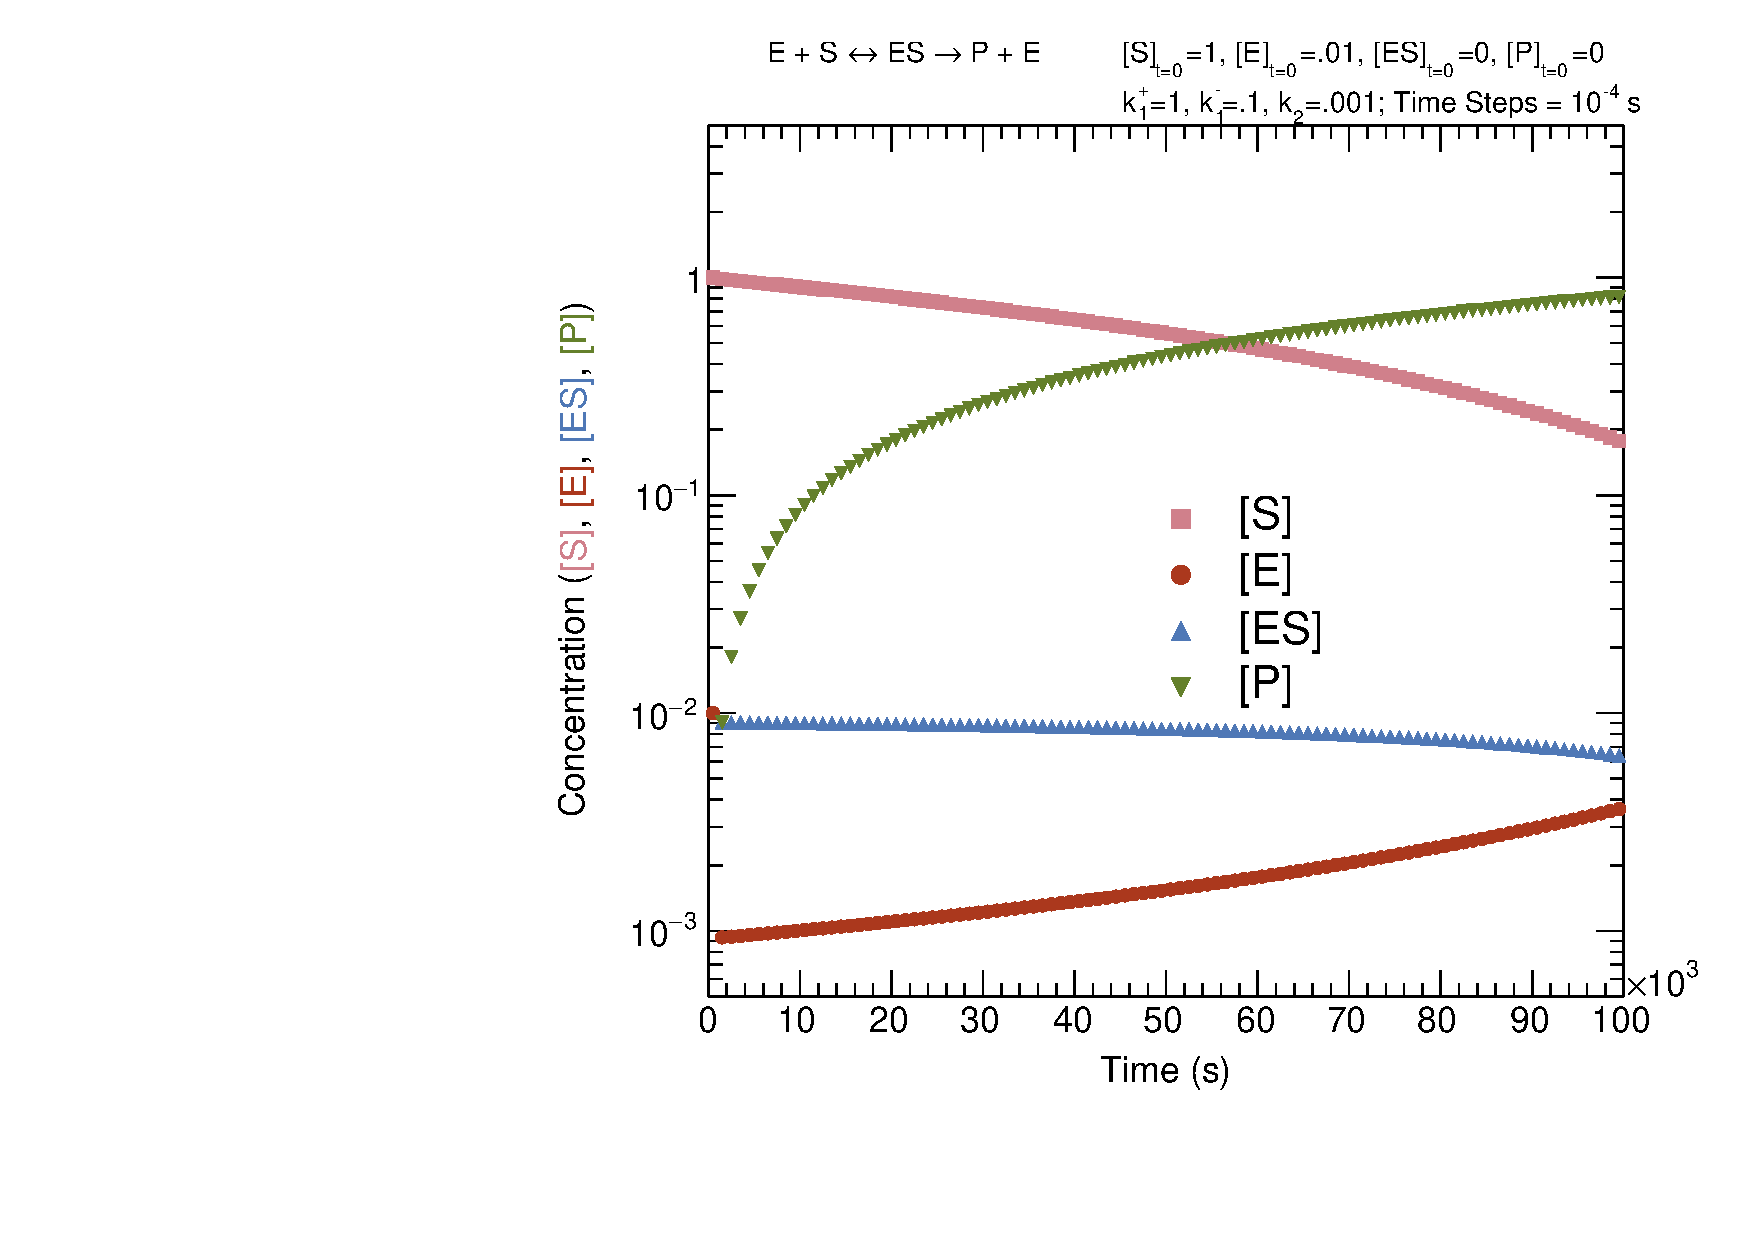
\includegraphics[width=.49\textwidth]{canv100k_c.pdf}
    \caption{Left: 0 $<$ t $<$ 5 seconds simulation, all concentrations. Right: 0 $<$ t $<$ 100,000 seconds simulation, all concentrations.}
    \label{}
\end{figure}

\begin{figure}[H]
    \centering
    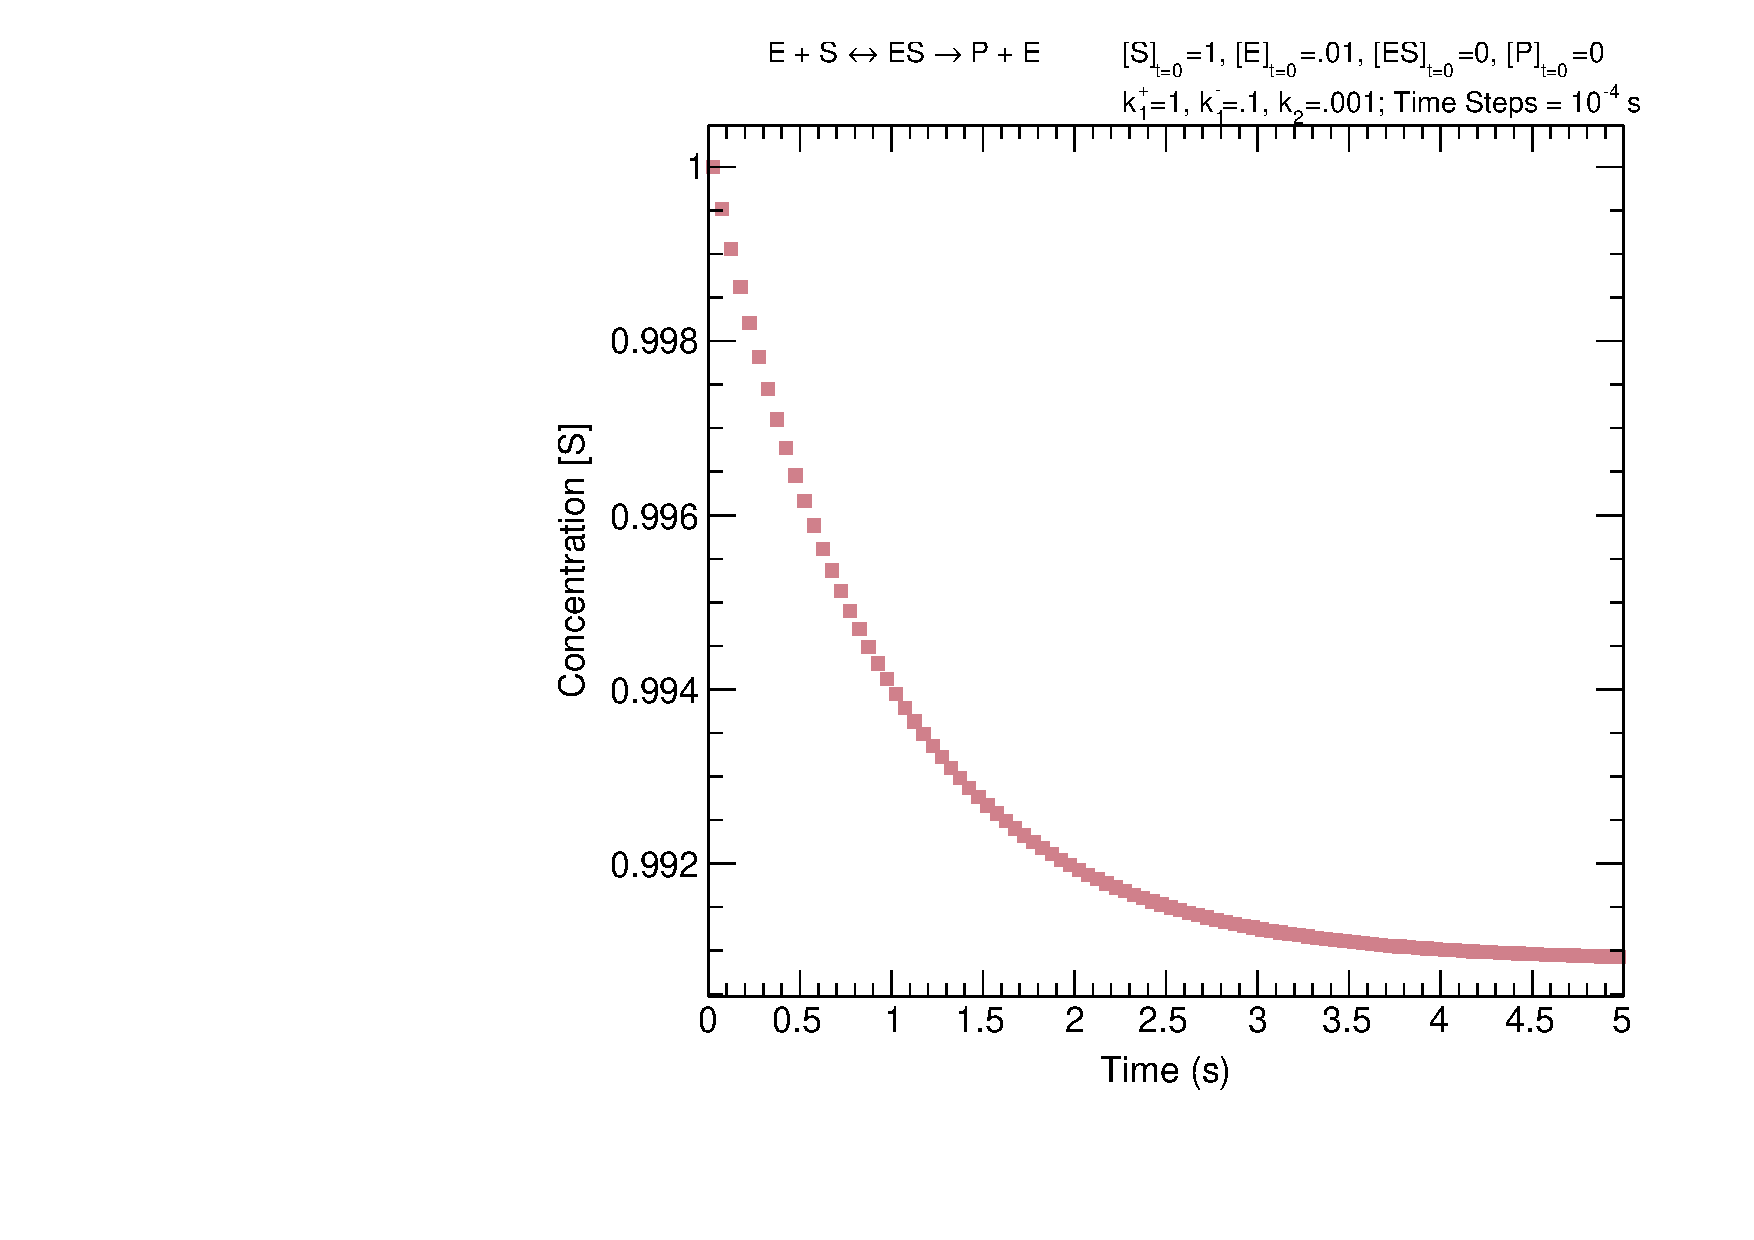
\includegraphics[width=.49\textwidth]{canv5_S_c.pdf} 
    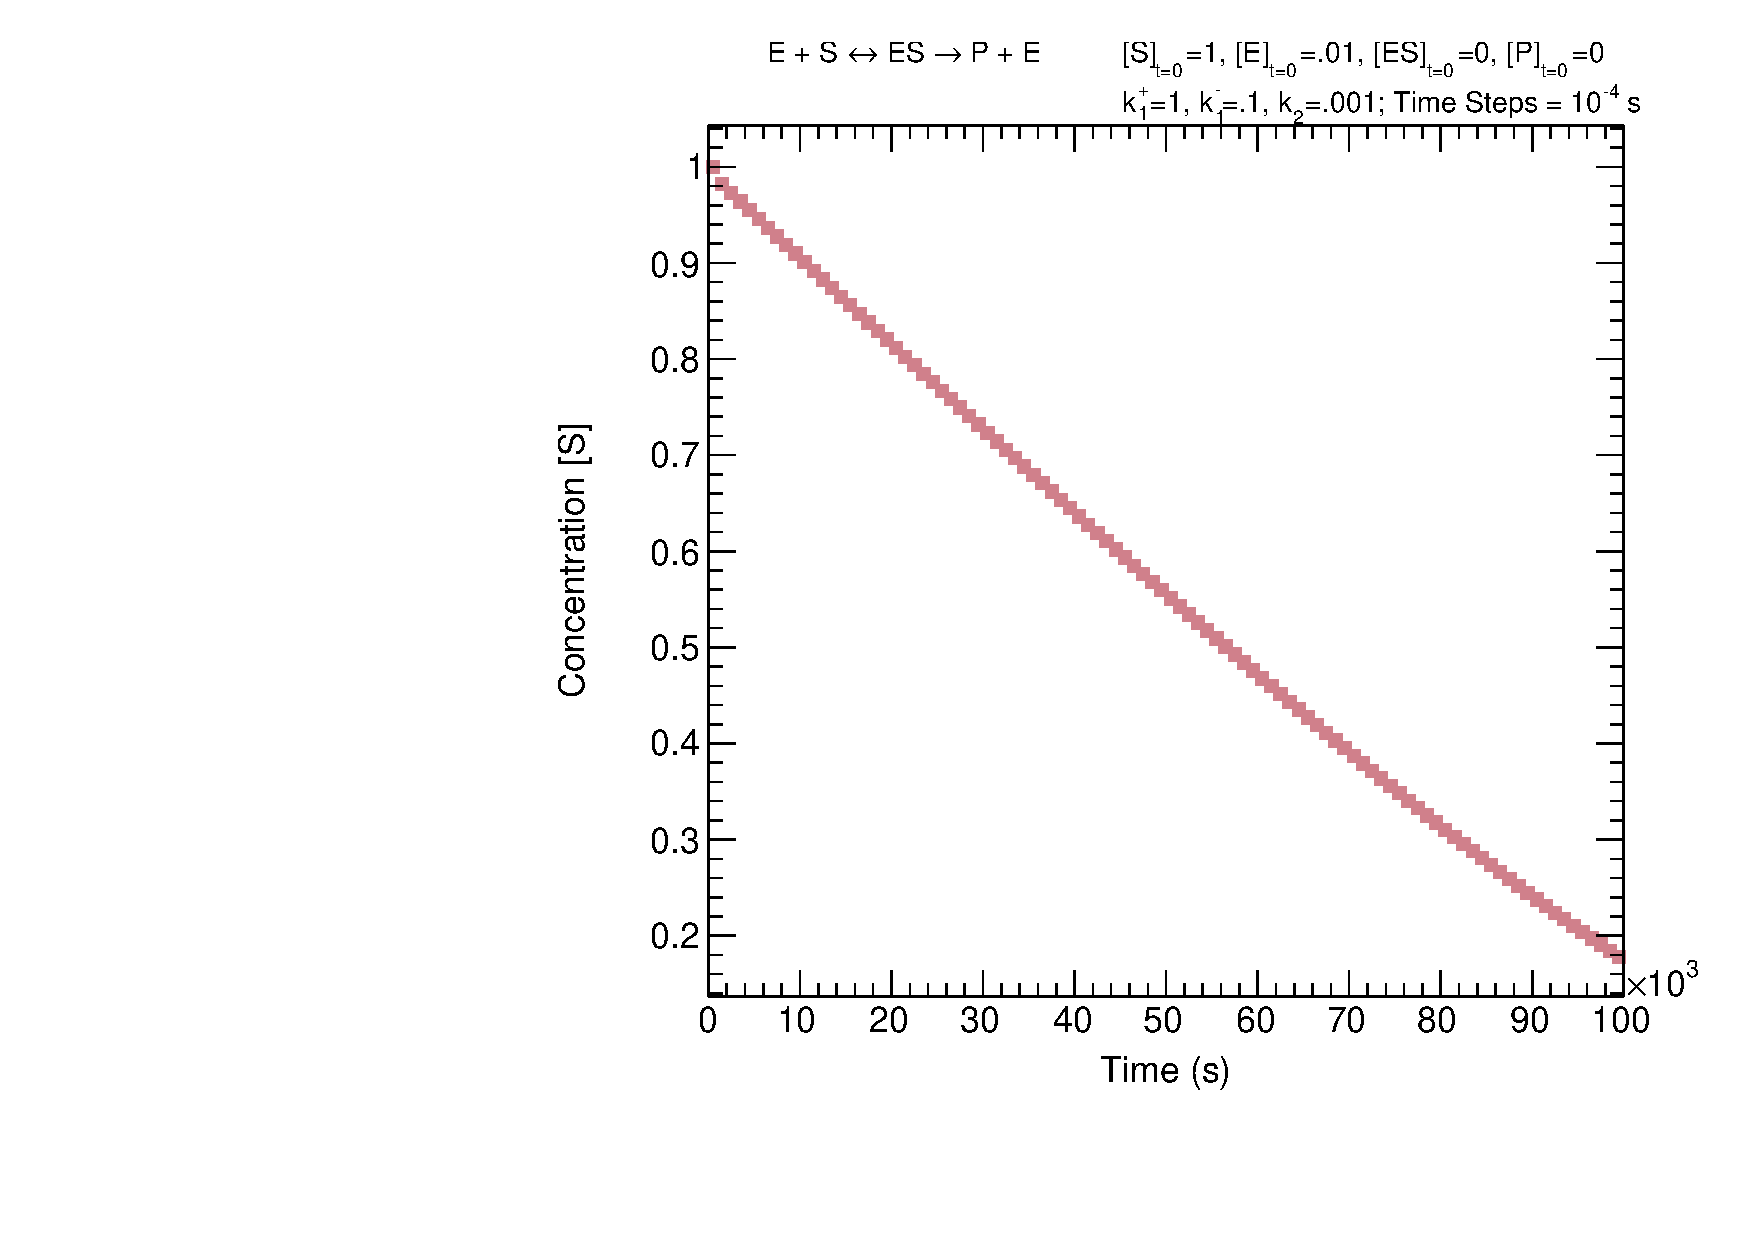
\includegraphics[width=.49\textwidth]{canv100k_S_c.pdf}
    \caption{Left: 0 $<$ t $<$ 5 seconds simulation, [S]. Right: 0 $<$ t $<$ 100,000 seconds simulation, [S].}
    \label{}
\end{figure}

\begin{figure}[H]
    \centering
    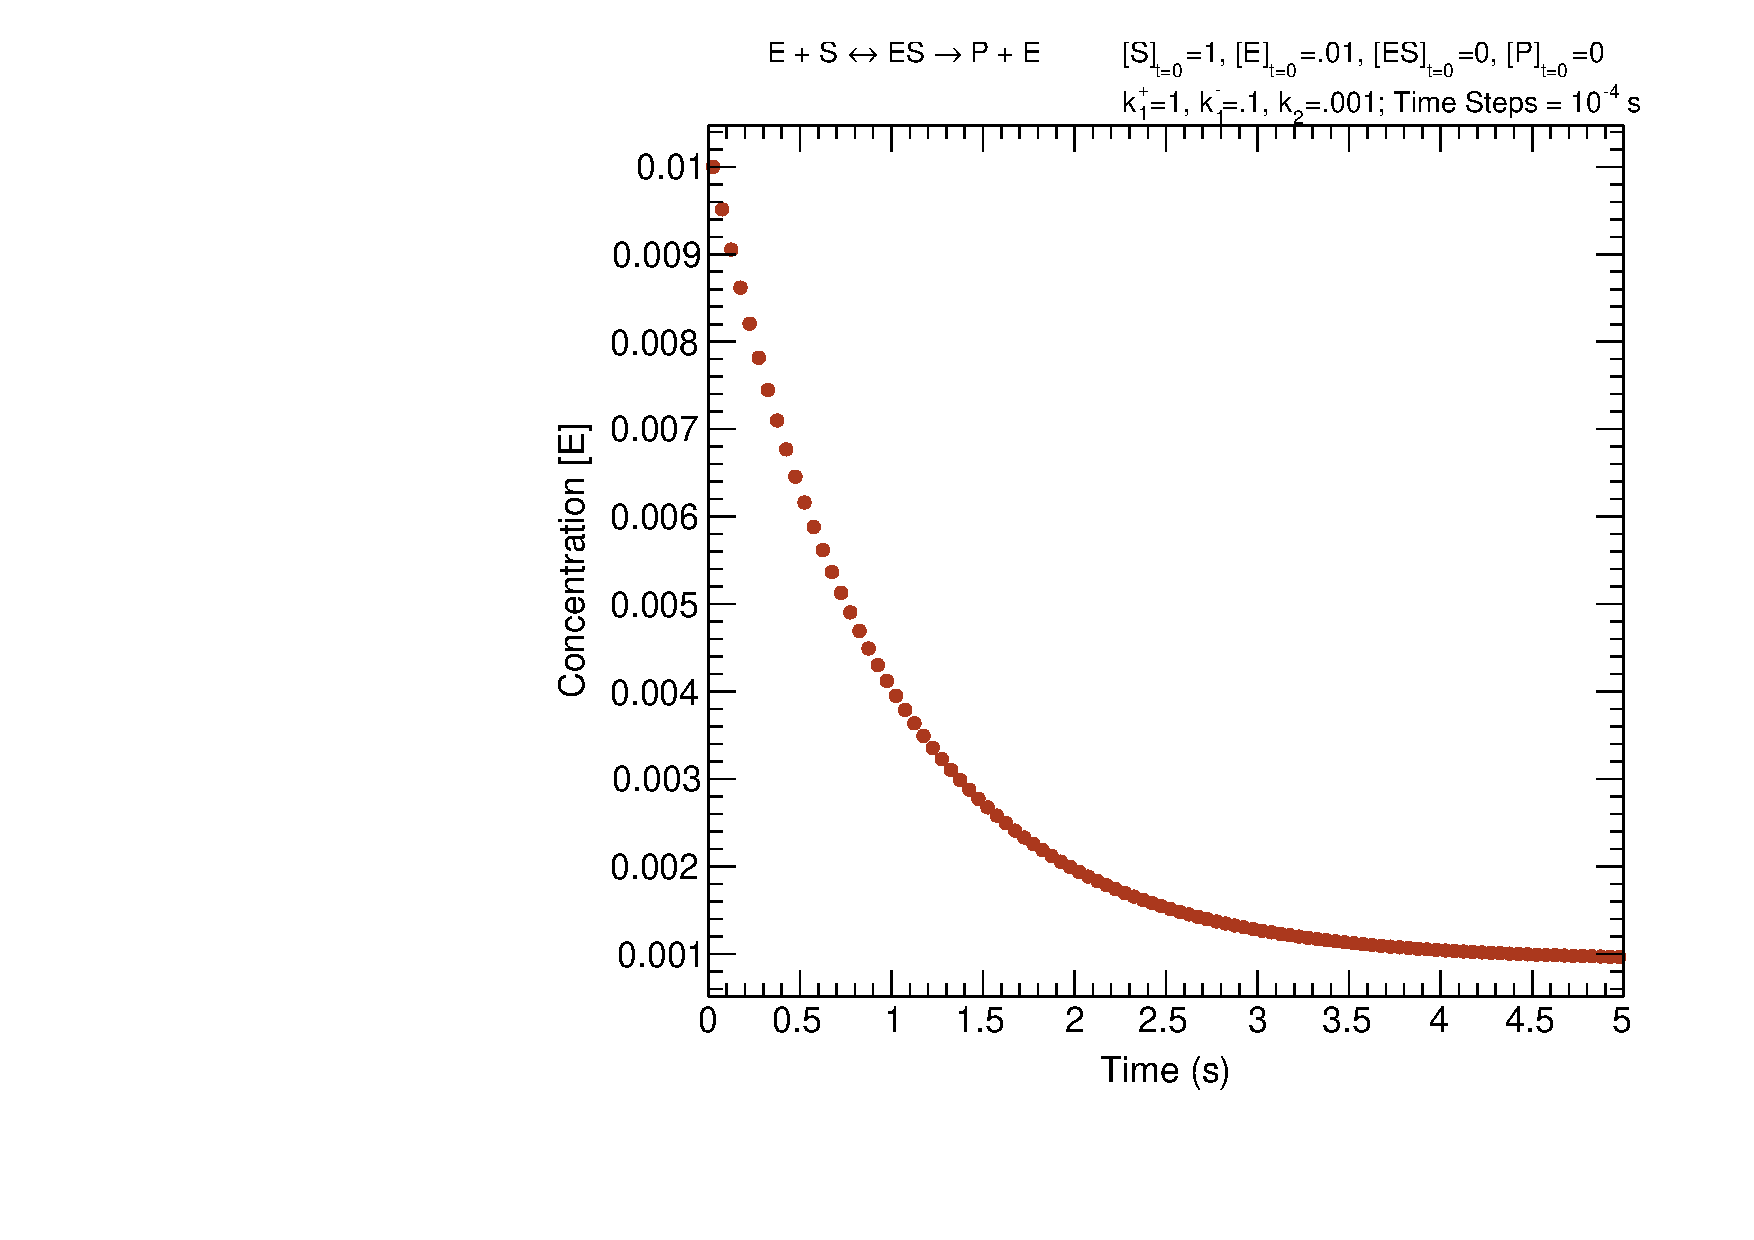
\includegraphics[width=.49\textwidth]{canv5_E_c.pdf} 
    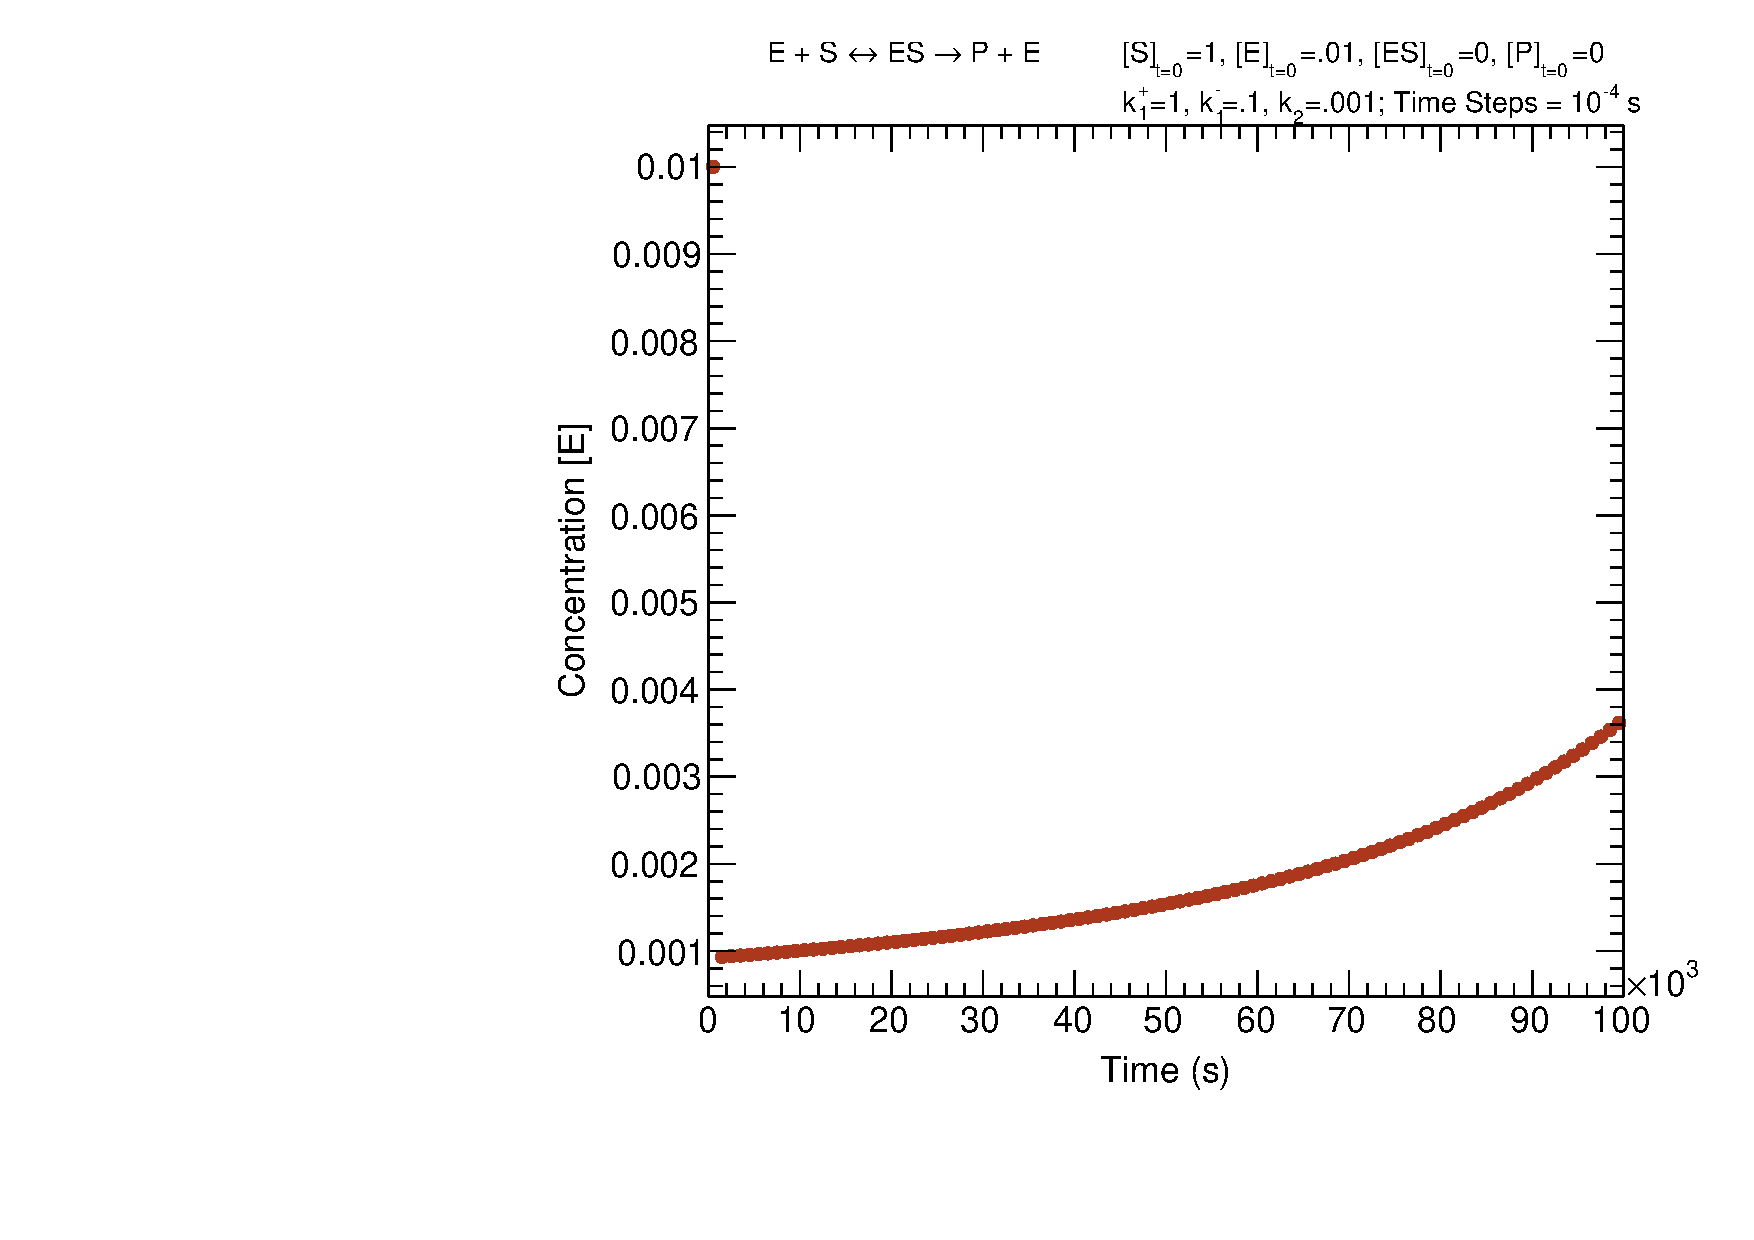
\includegraphics[width=.49\textwidth]{canv100k_E_c.pdf}
    \caption{Left: 0 $<$ t $<$ 5 seconds simulation, [E]. Right: 0 $<$ t $<$ 100,000 seconds simulation, [E].}
    \label{}
\end{figure}


\begin{figure}[H]
    \centering
    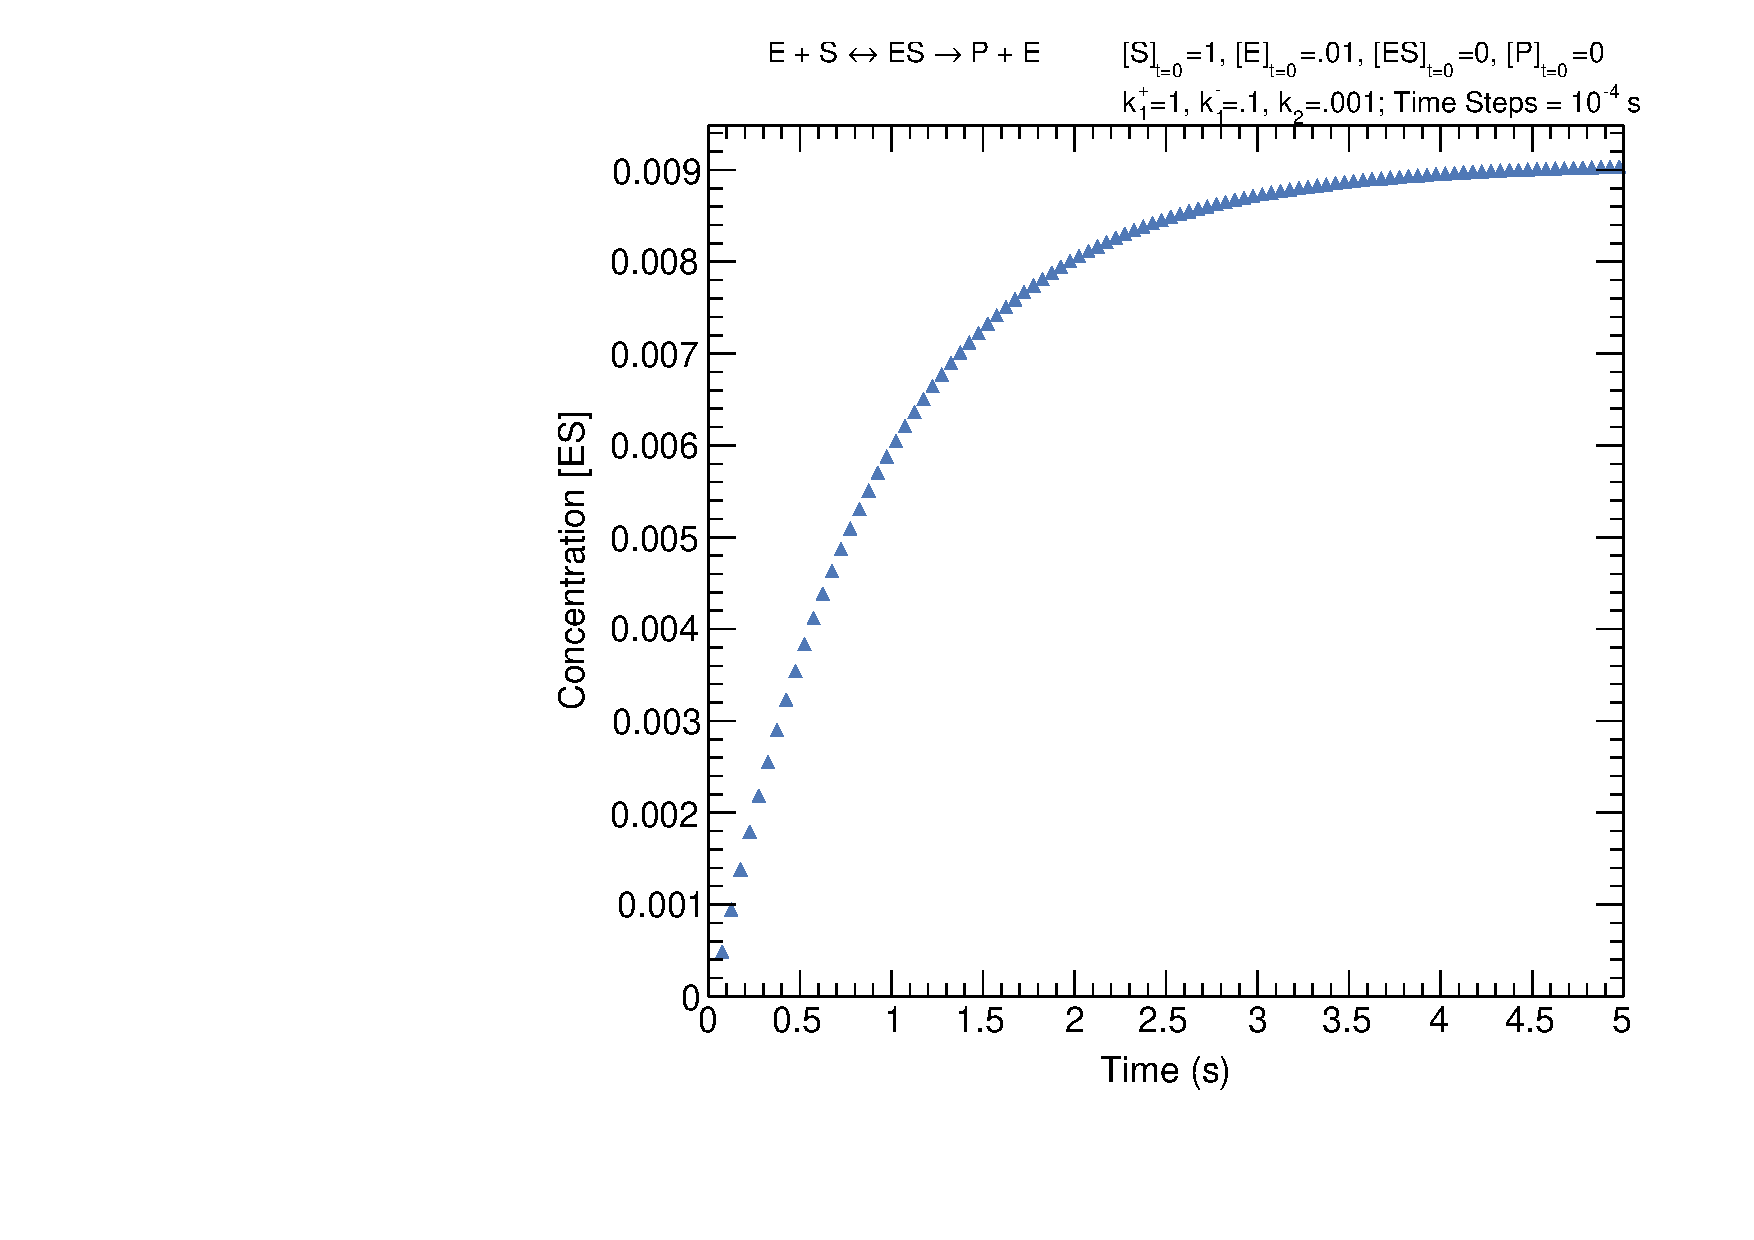
\includegraphics[width=.49\textwidth]{canv5_ES_c.pdf} 
    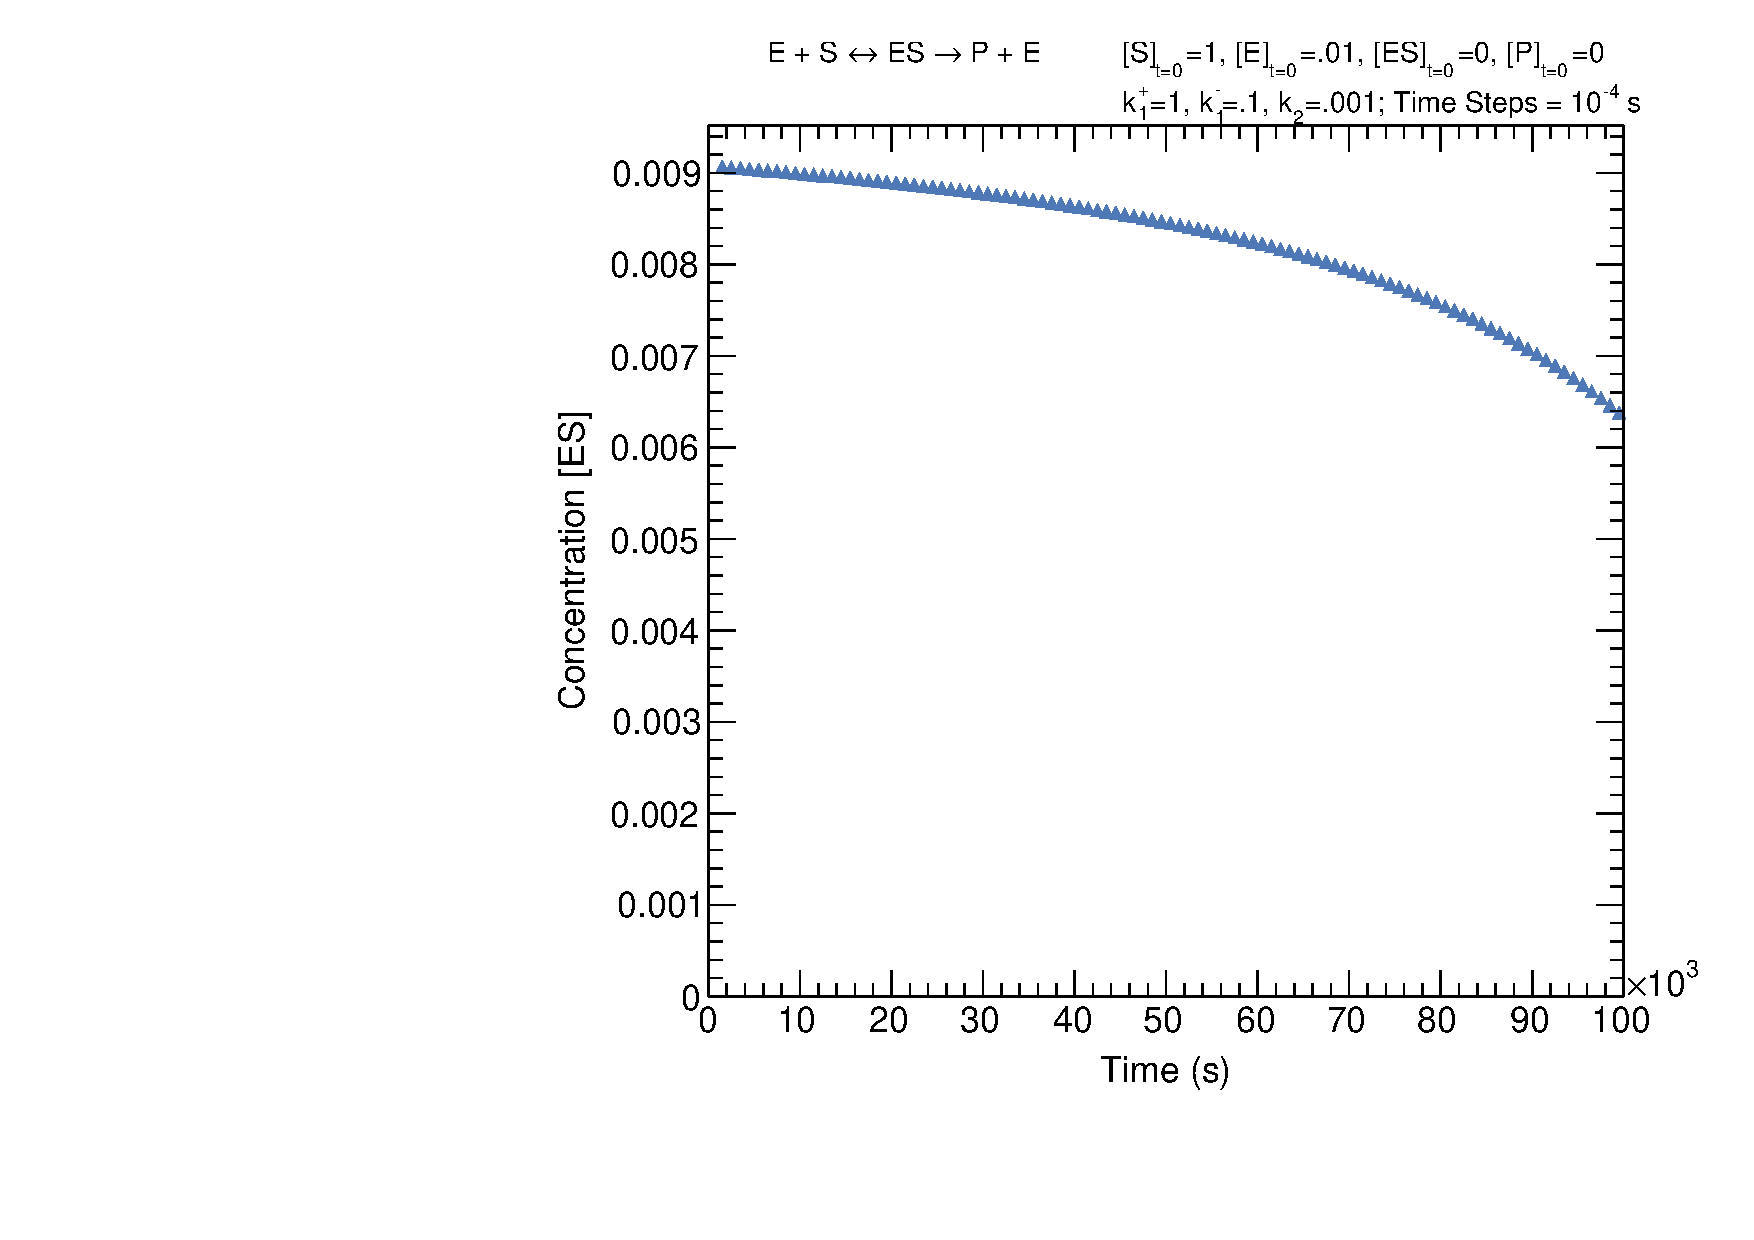
\includegraphics[width=.49\textwidth]{canv100k_ES_c.pdf}
    \caption{Left: 0 $<$ t $<$ 5 seconds simulation, [ES]. Right: 0 $<$ t $<$ 100,000 seconds simulation, [ES].}
    \label{}
\end{figure}

\begin{figure}[H]
    \centering
    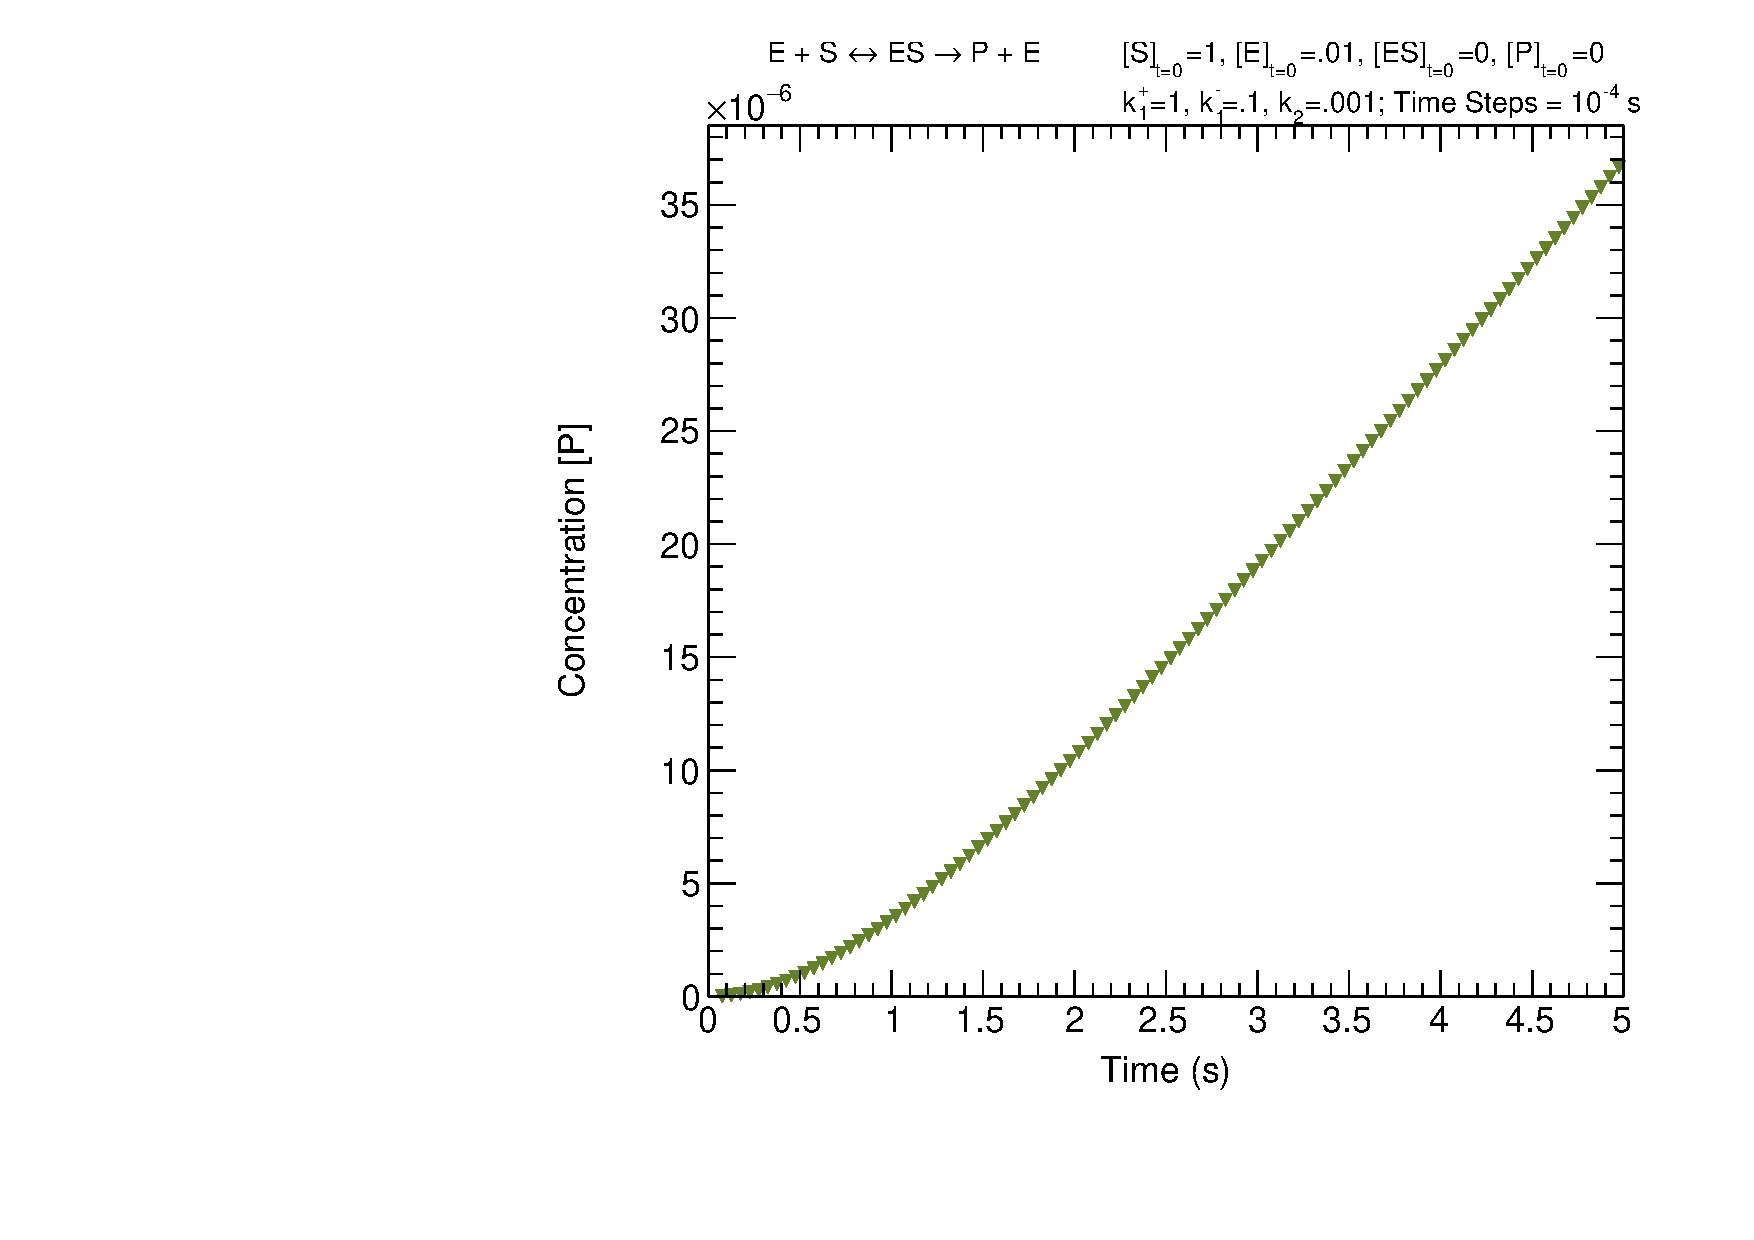
\includegraphics[width=.49\textwidth]{canv5_P_c.pdf} 
    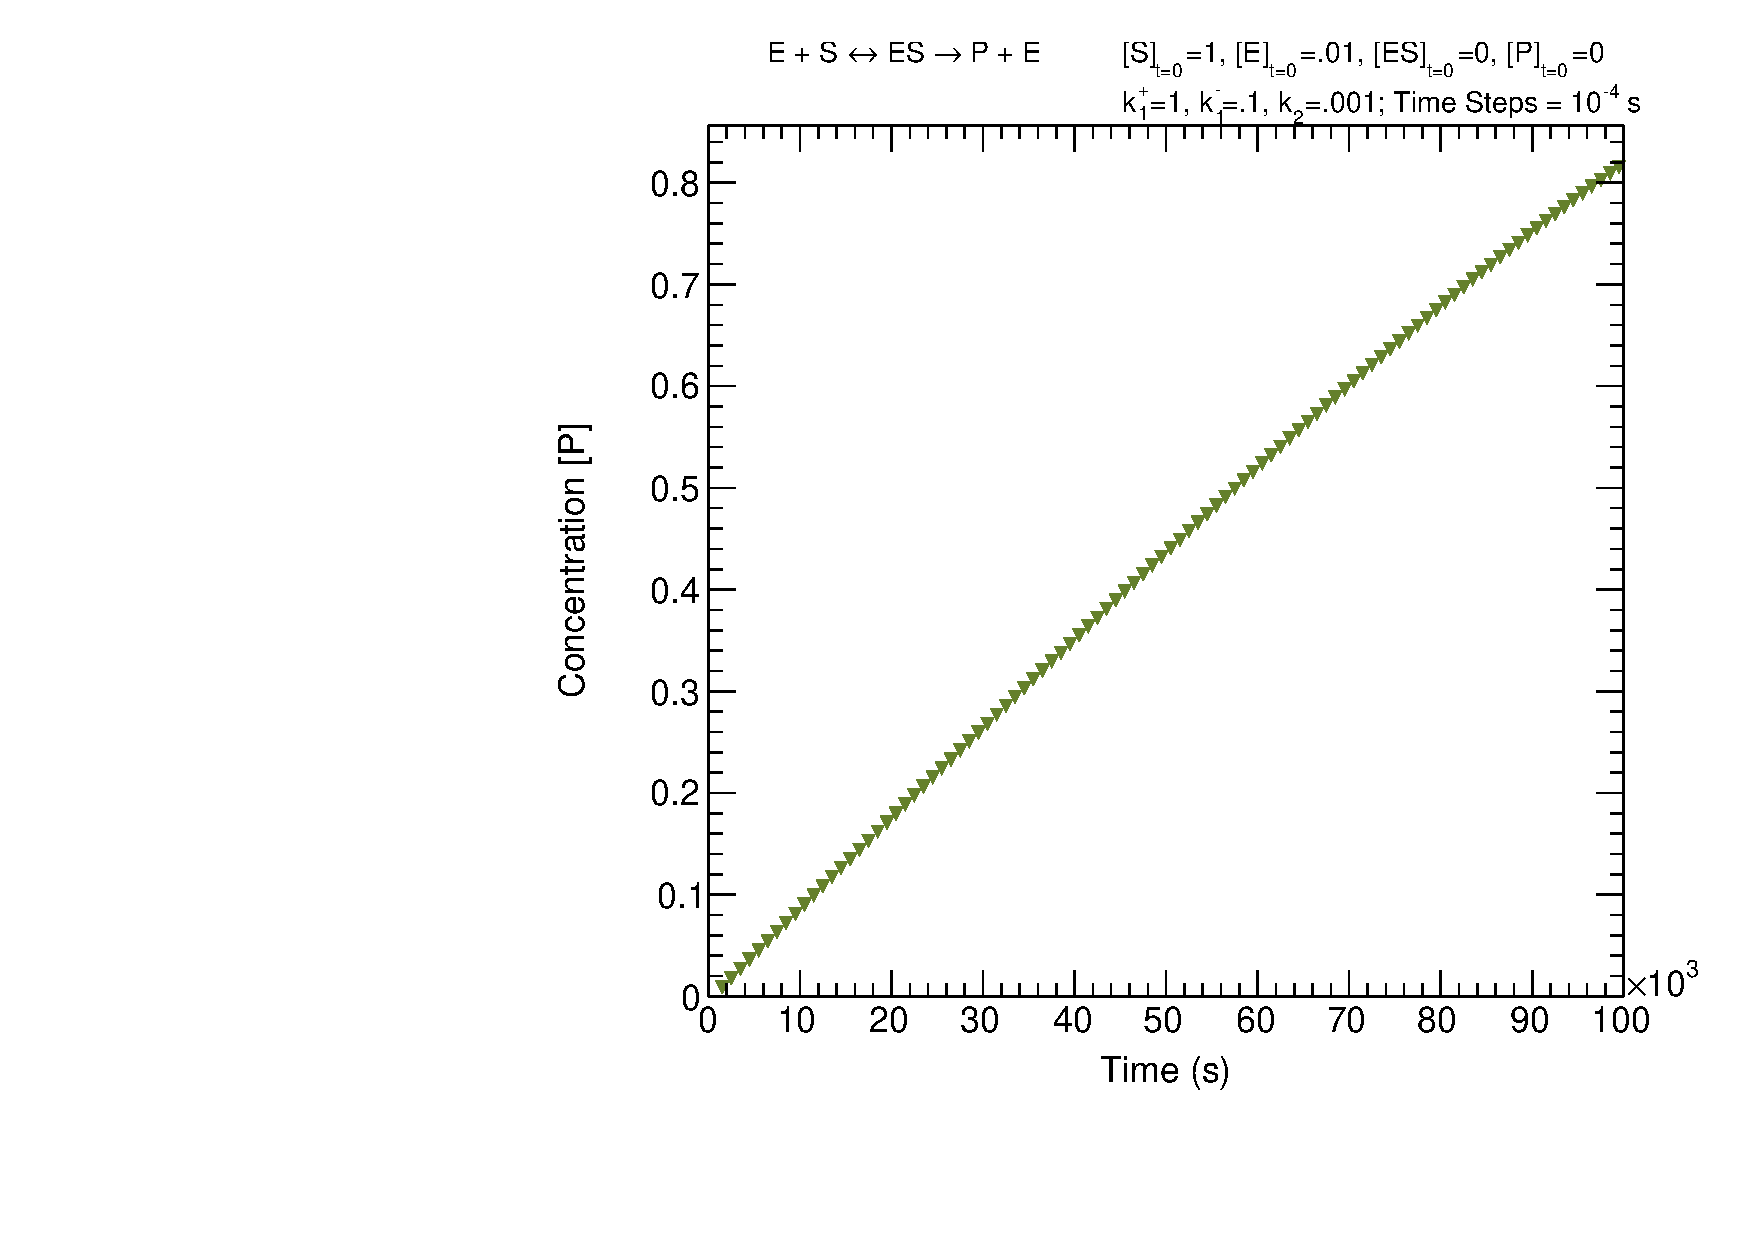
\includegraphics[width=.49\textwidth]{canv100k_P_c.pdf}
    \caption{Left: 0 $<$ t $<$ 5 seconds simulation, [P]. Right: 0 $<$ t $<$ 100,000 seconds simulation, [P].}
    \label{}
\end{figure}

\section{4.2.c}

\begin{figure}[H]
    \centering
    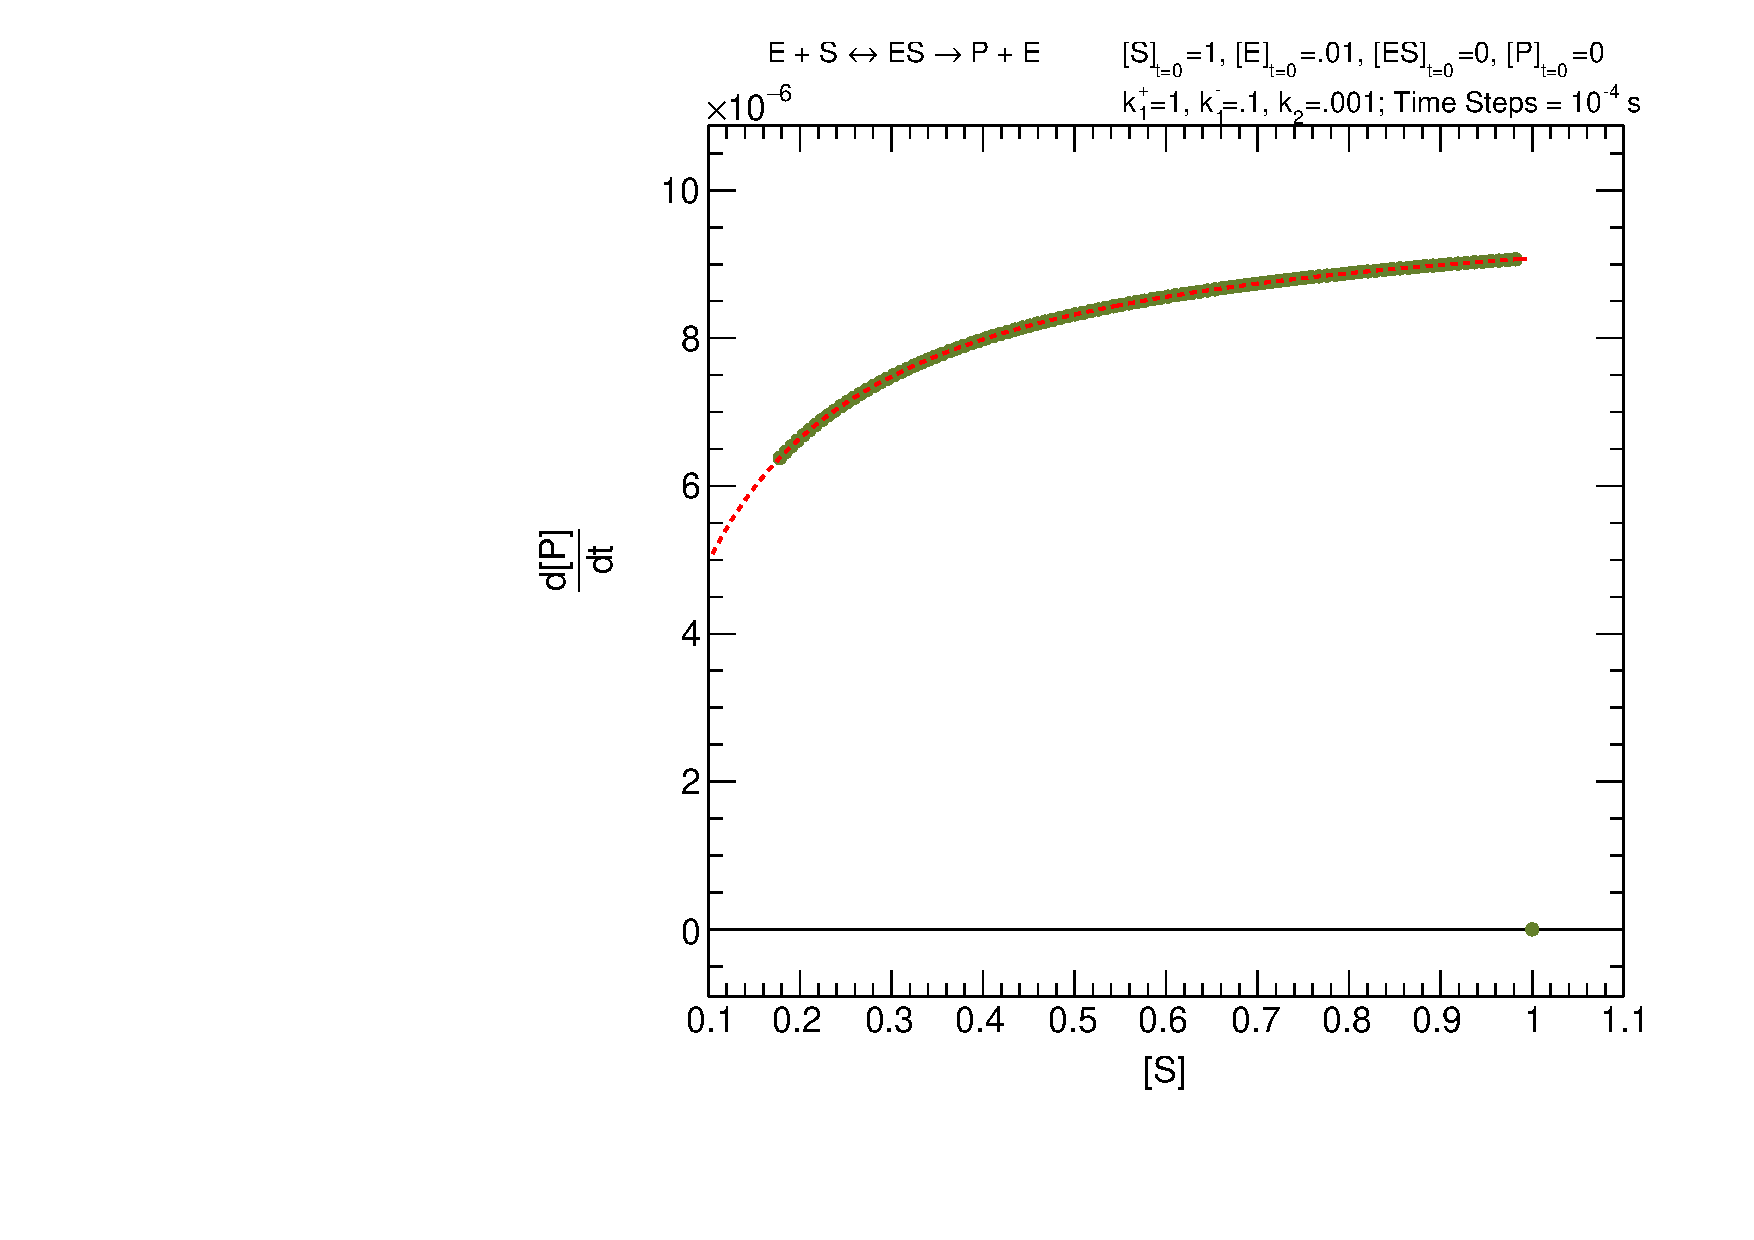
\includegraphics[width=.49\textwidth]{canv100k_PRate_c.pdf} 
    \caption{Production rate of [P] vs. concentration [S]. Note that the deviation from overlaid Michaelis-Menten (red-dashed curve) at [S] equal to 1 is because the system at that point has not yet reached quasi-equilibrium (see the corresponding set of t $<$ 5 concentration plots, rapid change on that epoch).}
    \label{}
\end{figure}

\section{4.2.d}
For half-time to quasi-equilibrium [ES], simulation gives $t_{1/2} = $ .6311 seconds, compared to my calculation of .63158 seconds, or within .07\%. Quasi-equilibrium starting value for [ES] is 0.00903606, compared to calculation of .00908, ~.5\% error.

For 100,000 second simulation, time to half [S] in simulation was 56094.1 seconds, compared to my calculation of 57764.7 seconds, for about a 2\% relative error. Overall agreement between calculation and simulation is quite good based on this set of comparisons.


\section{4c}
The following set of plots correspond to fits of data as specified in 4.3. Code can be found at github.com/cfmcginn/SystBio/HW1. C++ and ROOT needed to run. A directory containing the set of pdfs used in this document is available at the git repository, along with the .tex used to create this, if wanted individually. Fitting is done with a simple chi2 (see code for exact options used w/ ROOT TF1 class). 

\begin{figure}[H]
    \centering
    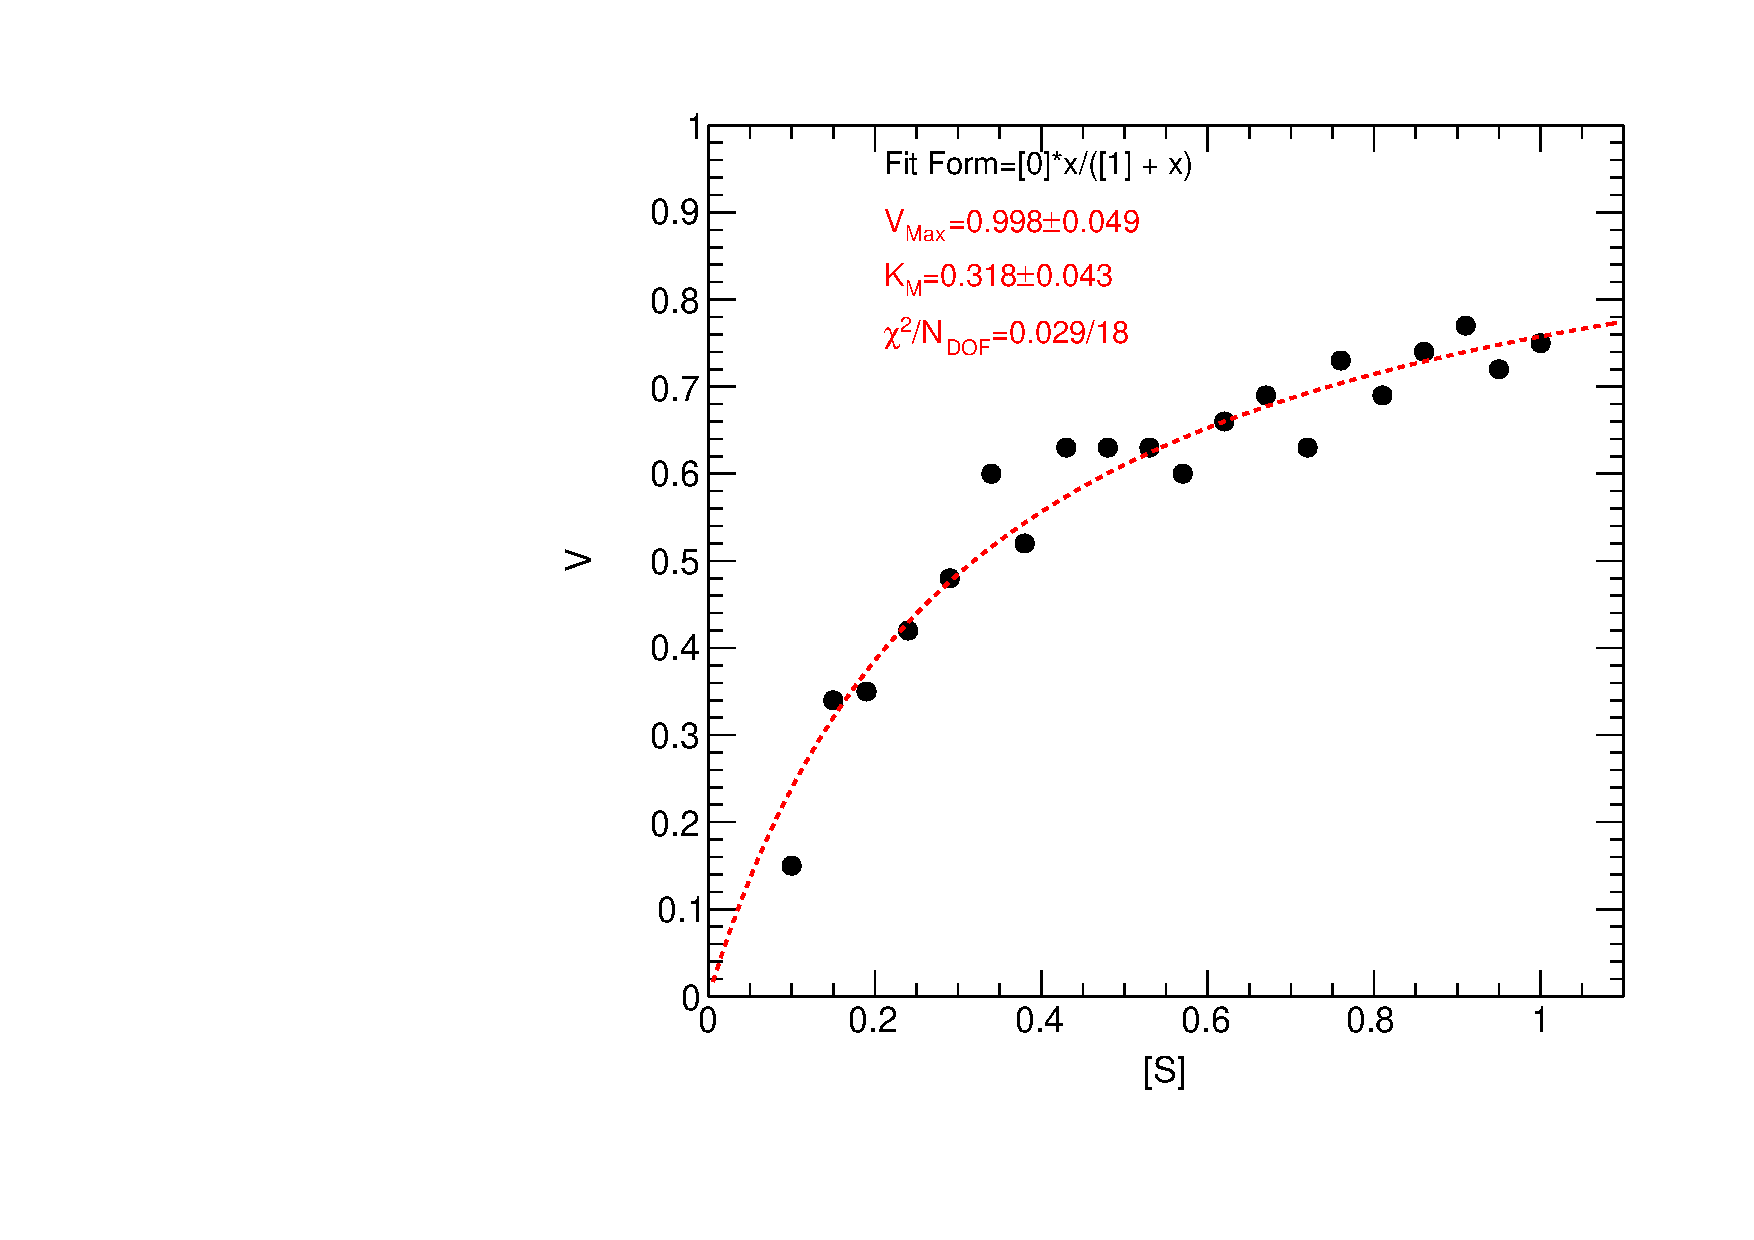
\includegraphics[width=.49\textwidth]{data1Fit_c.pdf} 
    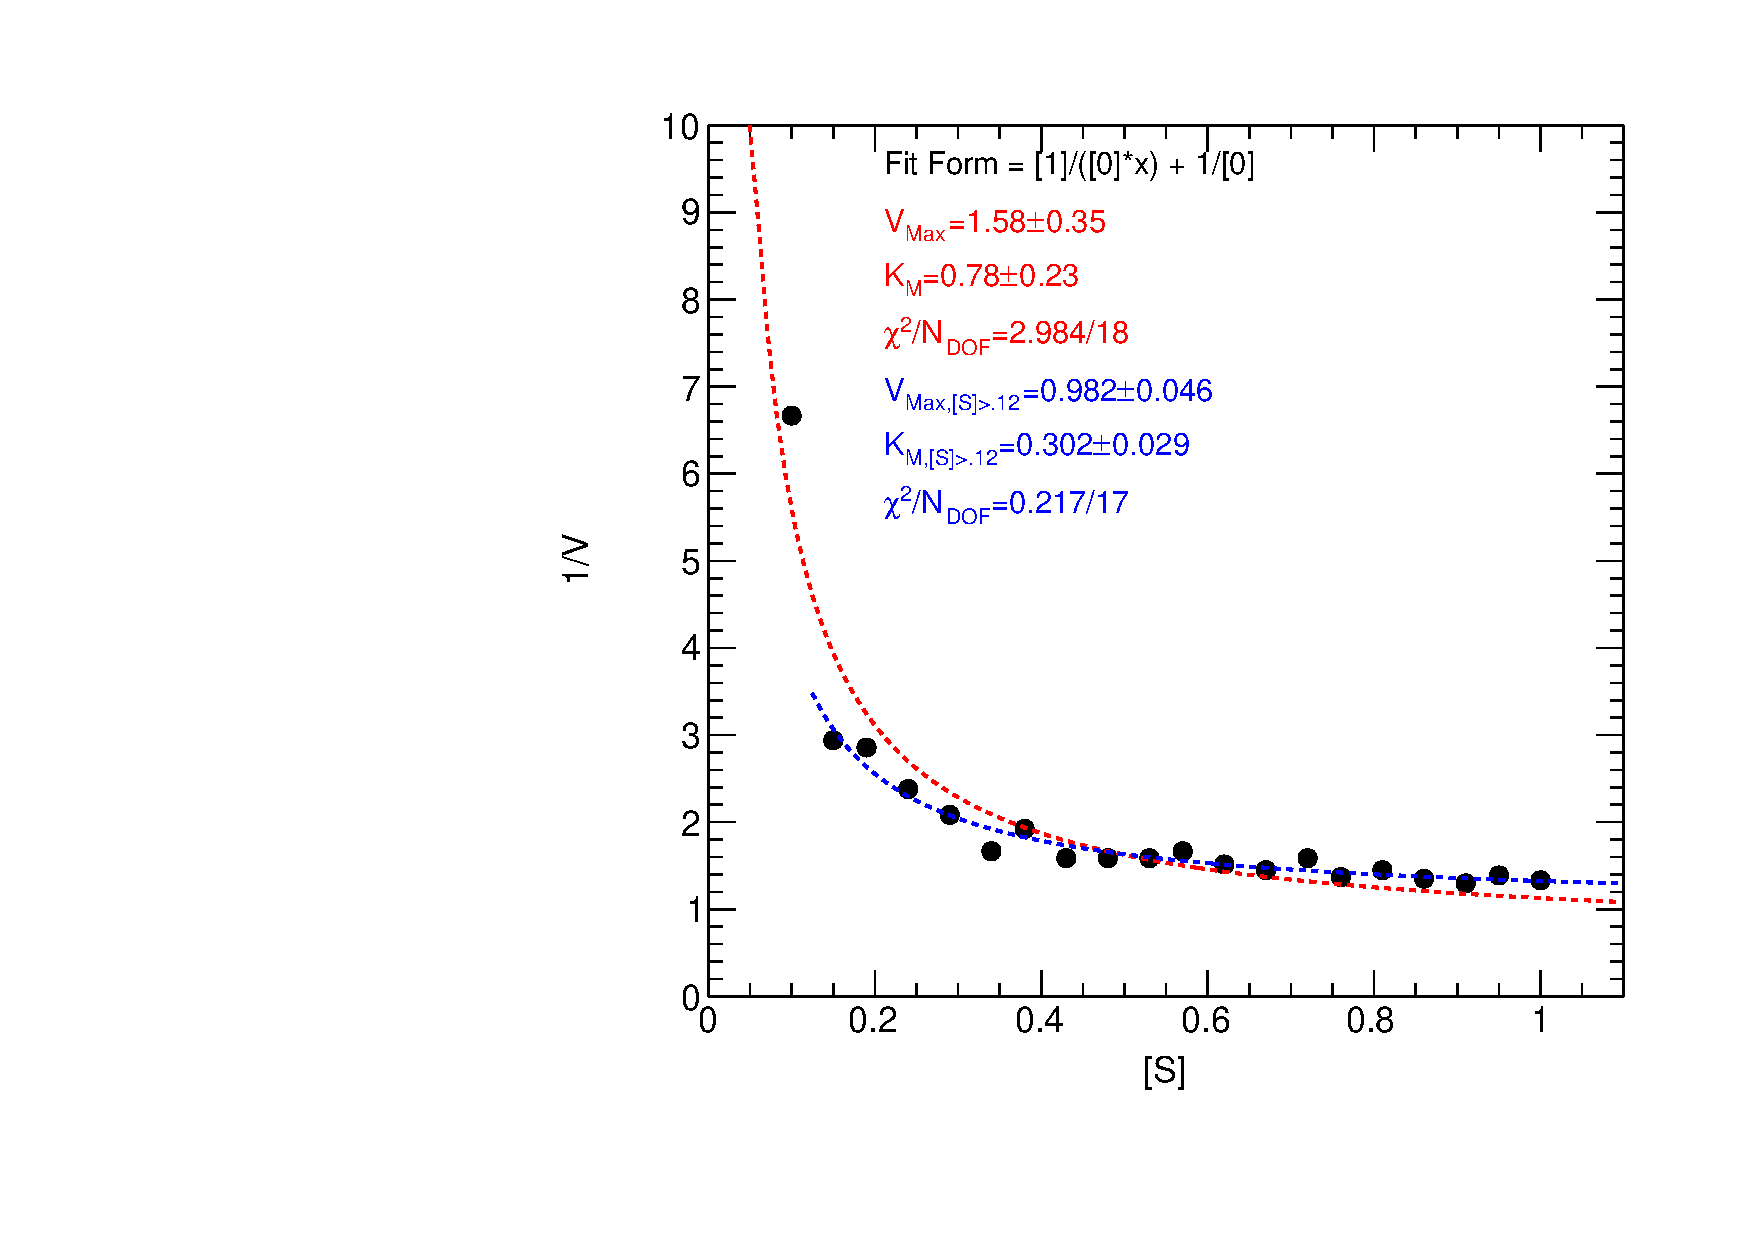
\includegraphics[width=.49\textwidth]{data2Fit_c.pdf}
    \caption{Left: Fit of standard Michaelis-Menten. Right: Fit of inverted Michaelis-Menten. Note: no errors were provided, so we are forced to fit with equal weights. The inverted Michaelis-Menten would return the same fit values if errors were included, as the point causing deviation would have large relative error (low weight) post inversion. Excluding that point in the truncated fit gives perfectly consistent parameters between left and right. Since difference is driven by a single point, which drives parameter errors up significantly, and point exclusion returns previous fit performance, it seems safe to say this is consistent, and inclusion of errors on data points would give consistent results over the full fit range again.}
    \label{}
\end{figure}

\end{document}

